\section{Sanje za Duso (Dreams for the Soul)}

\margininbox{13.8.12 - Milky Way}{

I don't know what to hope: That underground adventures with Tjaša
will become a tradition or not! Like last year (my first time down here)
we found the narrowest and the longest wet passages possible again. But
those places are also so beautiful, that I hope someone will discover
big chambers with a lot of new leads on the other side, and maybe a
shortcut to get there, so many of you will have the motivation to go
there and see what we saw! \name{Grega Maffi}}{\logbook}


\begin{pagefigure}
\checkoddpage \ifoddpage \forcerectofloat \else \forceversofloat \fi
   \centering
\includegraphics[width = \textwidth]{2012/sanje_za_duso/2012-08-13-1322-Maver-P8130192--orig.jpg}
\caption{Grega Maffi, Karin Rutar and Tjaša Rutar at camp \passage{X-Ray} on the final pushing trips of the expedition. \pic{Nejc Maver}} \label{slovs x-ray pushing}
\end{pagefigure}



The last pushing trip of the expo is always a bit extreme: we don't have
to reserve our energy anymore, so let's go with full power! It was
really great and exciting news that Mafi finished the climb of the
\passage{Apollo} in \passage{Queen's Bedchamber}, and at the top, yet
another phreatic passage was found, with some junctions that they did
not have time for checking out. So it was an obvious plan to go there.
In fact, at the top of the climb there were two possible continuations,
and the other one (at your back when you climb up) seemed to be even
bigger. So, my plan was to traverse across the top of the pitch to reach
this possibly large gallery. I managed to persuade Karin to give it a
go, and there we were, going down on the well-known route to
\passage{X-Ray}. Here we come, \passage{Vrtnarija}!

Of course, we were dreaming of the connection, or rather joking about
it. Karin said that she had a good name in her mind, which was also the
name of a hard climbing route that had been completed recently. But when
I asked her what it was, she replied that she can only say it if we find
the connection. So there we were, with a (hopefully) good name for a
passage that will only be given if it connects the two systems\ldots{}

After a good night sleep, and a healthy morning meal with meat and
tomato, we packed up all the gear for climbing the traverse: drill,
bolts, hangers, maillons, rope, and so on. Reaching the \passage{Queen's
Bedchamber} is a pleasant trip. There is one peculiarity though: at the
low passage in the chamber with the plenty of crystals, again there was
almost no wind. In the first year, when we found it, there had been a
huge draught here. Probably it was connected with the excess of water in
that time: almost all the big pitches had large waterfalls in them.
Nevertheless, we were certain that something big awaits us at the top of
the \passage{Apollo} climb.

I made my way up carefully on the rope. It was absolutely terrible. The
pitch was (and remains) the worst in the whole system; one can see the
heroic effort to reach the top, climbing through mud, montmilch\sidenote{moonmilk}, loose
rocks, and so on. Hopefully, a bypass will be rigged one day
here\ldots{}

Anyway, both of us managed to get to the top without killing ourselves
or the other, and we started the preparation for the climb. However,
just after I drilled the first hole, on cable of the drill came out
loose! There was nothing to do with it, so there we were, with all the
equipment, but without a working drill\ldots{} The climb was way too
long to be done with hand bolting. So what should we do? Well, let's
check out that junction that Mafi was talking about (and for which,
jokingly, I said that there is the connection :)

(The next year we did
the climb with Peter\sidenote{likely Peter Adamko, Gergely's friend and a fellow Hungarian}. Guess what? There is nothing on the other side!)

The passage leading there was nice, and soon we found ourselves at the
junction. Entering the passage, our good old friends showed up on the
wall: the wind-crystals! Hmm, so there used to be quite a strong draught
here\ldots{} let's see where it comes from!

We had to work on two squeezes for quite a while, especially that we did
not have a chisel, just a bolting hammer. But the crystals were always
there, showing us the right direction. (There was also a strange thin
material, like spider web or hair, in some places. Maybe that is formed
by bacteria, but it should be checked out\ldots{}) Moreover, as we
proceeded, we constantly checked the compass, and it \bignote{seemed that we are
heading directly towards the System}! The distance that we had to cover
was about 150 metres.

The passage was small, at one squeeze I had to take off my SRT to pass
through. Finally, after negotiating yet another squeeze, we entered in a
big space! It was a rift, about 25 m high, and checking the direction,
we were certain that we managed to get to the continuation of the
\passage{Minotaur Rift}-\passage{Guillotine} fault line. So, the game was on!
We climbed up in the rift towards \passage{Guillotine} in order to have a
look, but that was not the goal why we were here\ldots{}

\margininbox{Sanje za Duso}{
     \begin{itemize}
    \item Gergely Ambrus
    \item Karin Rutar
    \end{itemize}}{\explo}

Just as in the fairy tales, a nice open passage started from basically
the point where we emerged in the rift. Its direction was right towards
the system! Our distance at this point was about 50 metres. There was a
draught and crystals, so we became quite excited\ldots{} We started to
follow the passage. Then a climb up, then\ldots{} it is blocked here!
Hmm, a dead end. But going back to the passage, we noted that it
actually has more levels, it was a phreatic meander. We could pass one
level below, then again up, then again down, then\ldots{} we ended up in
a passage which lead to the side of a fairly big pitch with a
waterfall! By that time, I knew the description of \passage{Waterloo} by
heart, so I became very curious. There was a small ledge, about 30 cm
wide, on the right hand side of the pitch, going across (maybe 5 m
long). Luckily, we had some rope and maillons, so I started off from a
natural, and proceeded carefully along the ledge. Then, in the middle,
\bignote{where I had to step down, I saw\ldots{} two rusty spits!} So, there it
was, there we were: the result of so much effort by so many people, on
the last pushing day of the expedition, following the wind crystals, we
got into the system!

I called out to Karin. ``Hey Karin, what is the name that you had in your mind?''

``What?''

''Well, you better remember the name, because
there are two rusty spits here!''

At the beginning, she did not want to
believe it, but after I got to the other side and fixed the rope, she
saw it herself. We stood for a minute, still not believing what
happened. On the other side of the pitch, there is a nice big chamber
(\passage{Waterloo}), and soon we found the PSS 13 from Dave Wilson and
Andy Jurd, who have been here in 1998. We built a huge cairn, and placed
a sign, stating the exact date and time, and the fact that \passage{System
Migovec} became the longest cave system in Slovenia! And the name?
\passage{Sanje za Duso}, which means \passage{Dreams for the Soul}\ldots{}
really an aptly named passage!


\fullwidthbox{14/8/2012 1:15 am - The Connection!}{
Long John time! We deserved it, we pushed the \passage{Vrtnarija} for 70m (that’s what Gergely said) down. That means also that we found around 12km “new” cave -> it has a name -> \passage{Sistem Migovec}. I still can’t believe it.

We wanted to bolt to the right window in \passage{Queen's Bedchamber}, but the drill broke. That’s why we went up left into \passage{Milky Way} to check out the unpushed passage. The direction and draft (+ cristals) were showing us that we’ll get somewhere near Sistem. But we didn’t expect that we’re going actually find the connection.

Gergely said that we had luck. For a few moments I also believed so (that’s when I saw the PSS13 – \passage{Waterloo}) but I don’t believe in luck. OK there is possibility that we had luck, but that’s just a rare moment when you can’t explain it differently than saying it was luck (if you ask me). However I don’t care what it was, we found the connection and both of us are very happy.
\name{Karin Rutar}}


Fate is a strange thing. If back in 1998, instead of descending down
\passage{Waterloo}, they had traversed the pitch and followed the passage
that we came through, they could have found basically the whole
horizontal development in \passage{Vrtnarija}. On the other hand, we would
probably not know \passage{Concorde}, \passage{Pico}, or \passage{Happy Monday}.
And also, we could not have found the connection, and could not have
this story either.

What happened after? We carefully surveyed everything of course.
Descending down the \passage{Apollo} climb was just as bad as climbing up.
Back in \passage{King Minos} palace, we admired the crystals one more time,
now knowing for sure that indeed, there was something big behind them --
namely, a system of at least 12 km of caves! Back at home, in
\passage{X-Ray} (which was 70 metres lower now than in the morning), we
decided to celebrate by a candlelit dinner, and by finishing off our
whisky reserves. So we made one hot chocolate whisky after the
other\ldots{}


\begin{figure*}[t!]
\checkoddpage \ifoddpage \forcerectofloat \else \forceversofloat \fi
   \centering
\includegraphics[width = \textwidth]{2012/sanje_za_duso/2012-08-14-1852-JanaCarga-360--orig.jpg}
\caption{Freshly out of the cave, smiling widely, Jim and Gergely (Karin approaching) shake hands over achieving the connection. \pic{Jana Čarga}} \label{connection handshake 1}
\end{figure*}

As a result, the next morning I was in terrible shape,
although Karin did not have any problem. Strong girl! We started to pack
up, enjoyed the last solitary time before the transporting team arrives,
and then the news started to spread -- the connection has been found!
Big celebration on the surface, media, party -- but that is another
story. Jonny's final entry in the logbook for 2012: ``So, an ordinary
derig was made much less ordinary when Gergely + Karin told me that the
cave is now 70 m deeper. Hooray for sys-mig.''

It was a moment that is going to stay with us for our whole life. But I
particularly like it because it really has been the result of the effort
of the whole group, over so many years. We had been lucky to have the
chance of being there -- but we had been even more lucky to belong to
such an excellent team of nice friends.

\name{Gergely Ambrus}

\begin{pagefigure}
\checkoddpage \ifoddpage \forcerectofloat \else \forceversofloat \fi
   \centering
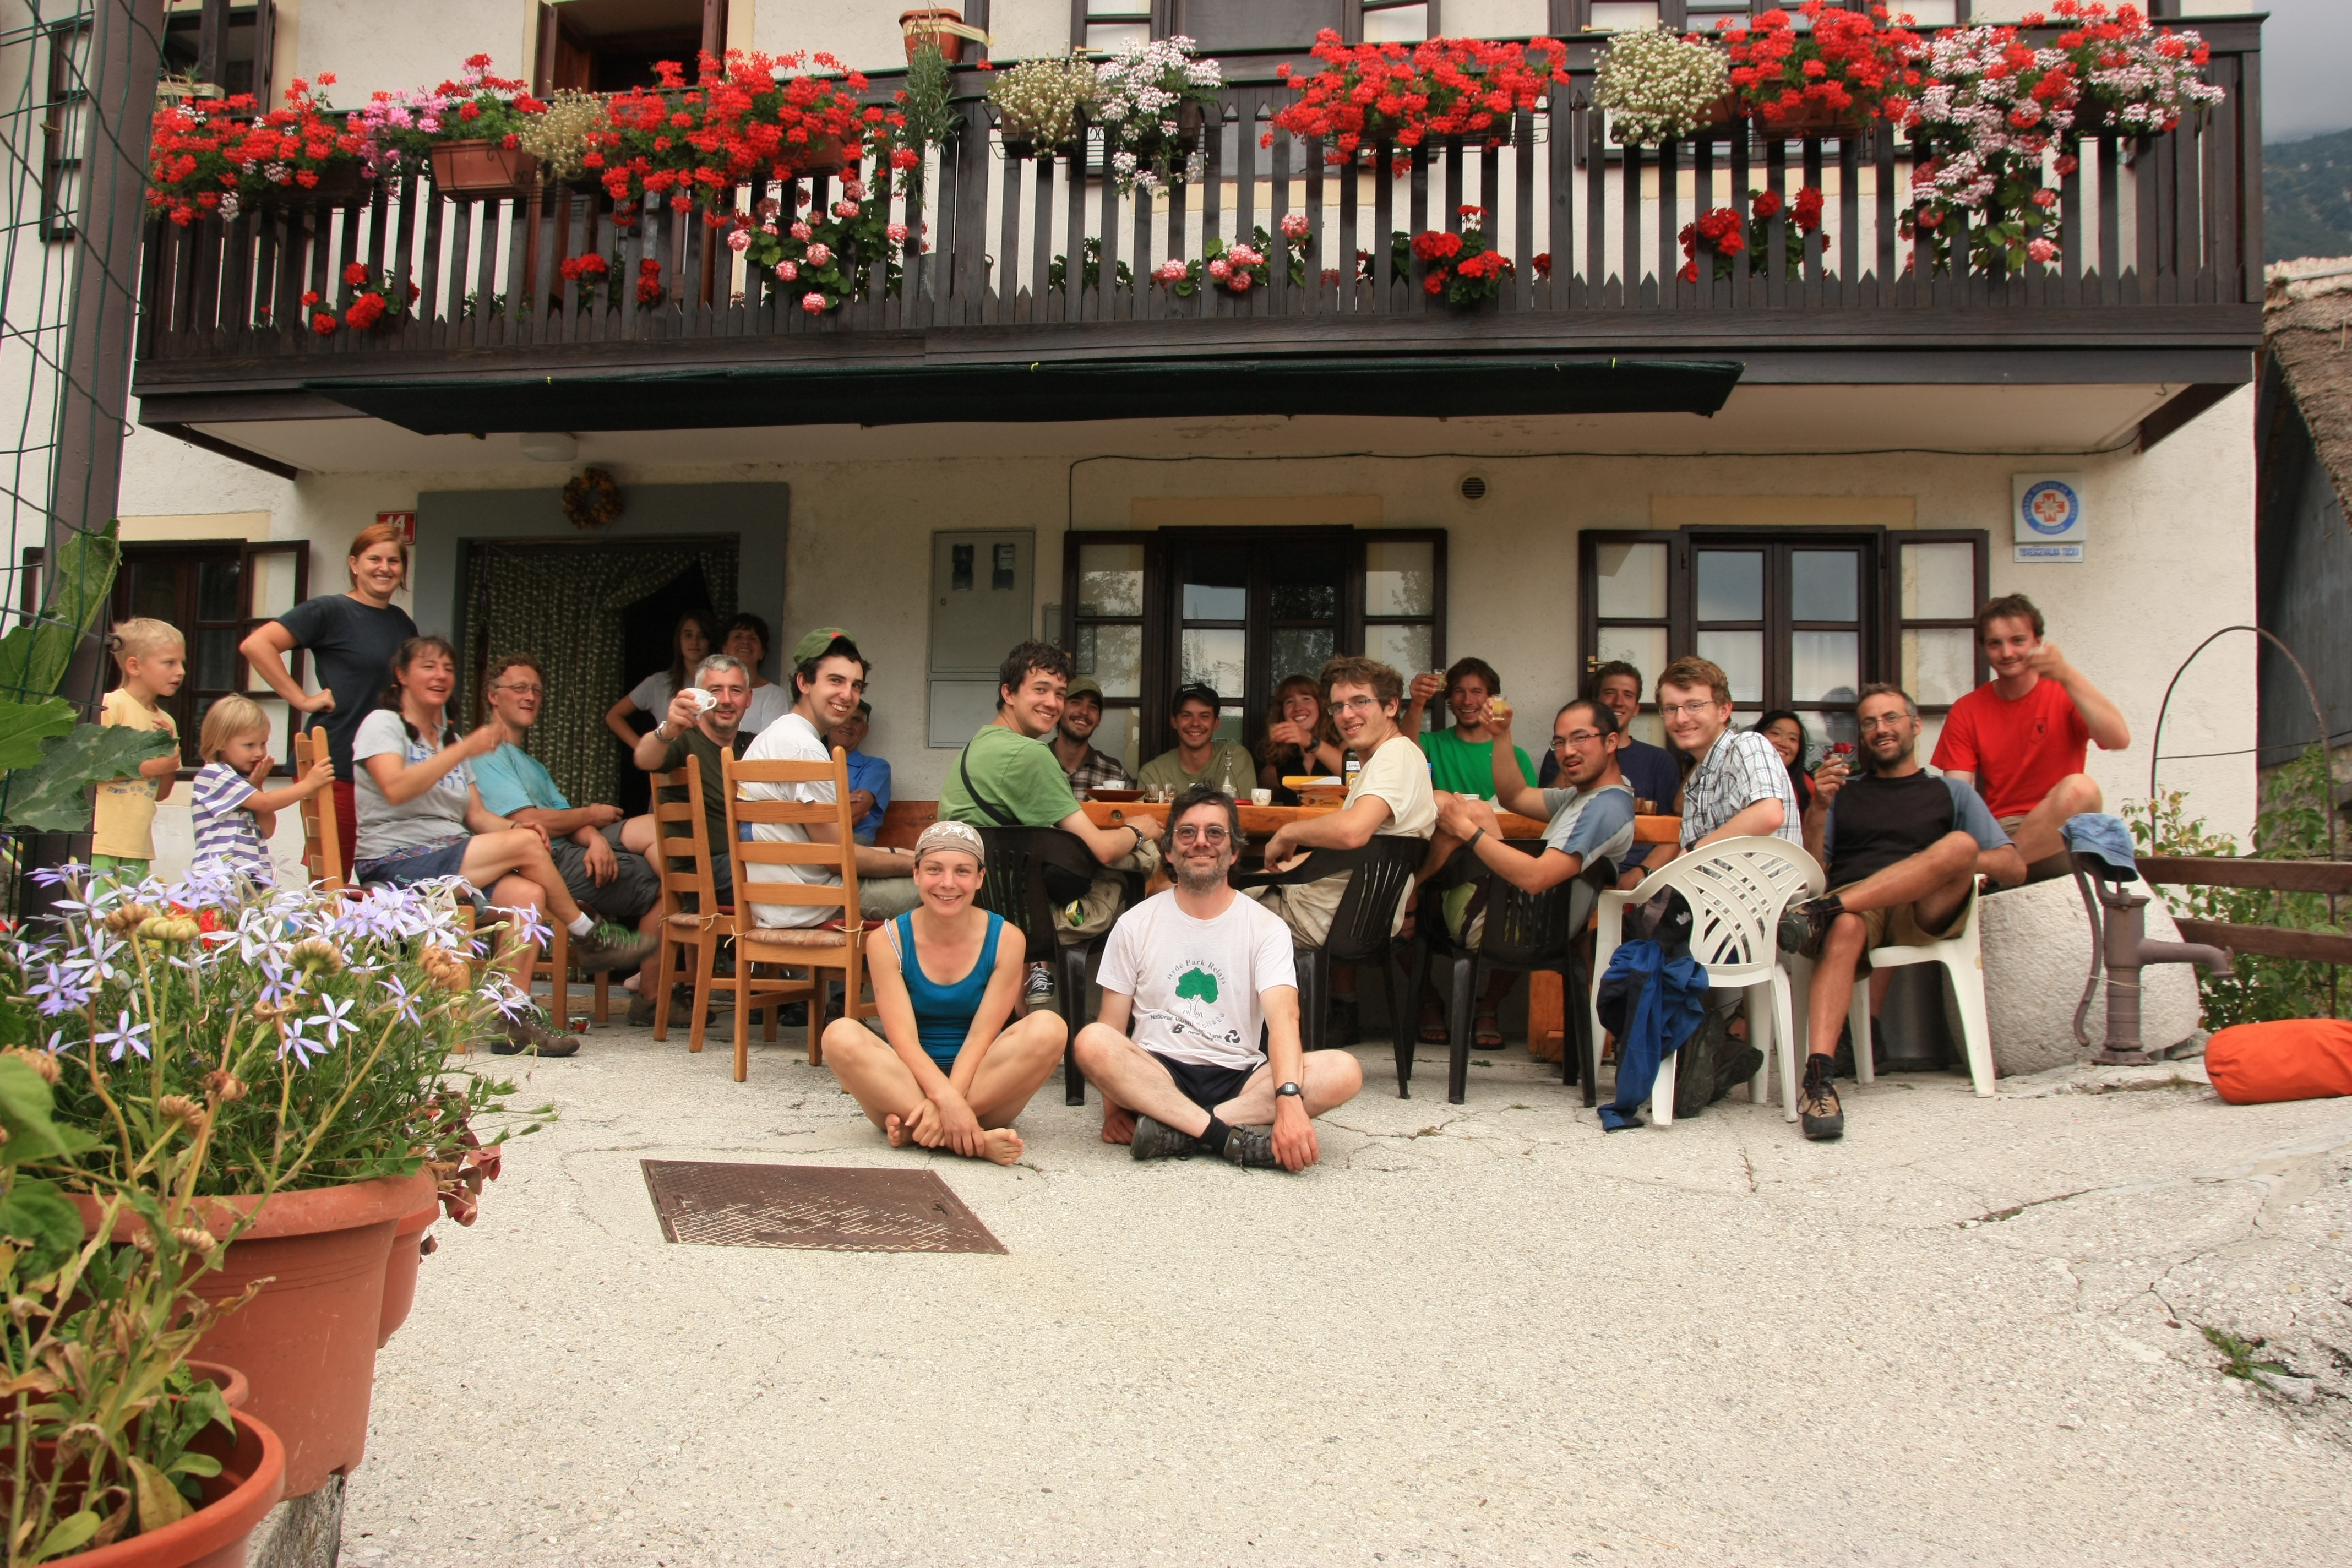
\includegraphics[width = \textwidth]{2012/sanje_za_duso/2012-08-16-0651-JanaCarga-532a--orig.jpg}
\caption{The team outside the Klobučar house after the final down-carry. \textit{left to right} Nada Klobučar, Janet Cotter, Jim Evans, ??, Martin McGowan, Slavica Klobučar, Saber King, Marjan Klobučar, Jana Čarga, Rhys Tyers, Iztok Možir, Nejc Maver, Dave Wilson, Kate Smith, Oliver Myerscough, Gergely Ambrus, Tharatorn Supasiti, Tim Osborne, Sam Page, Clare Tan, Tetley, Jonathon Hardman. \pic{Jana Čarga}} \label{2012 expo photo}
\end{pagefigure}